\subsection{DR25 KOI Catalog Completeness and Reliability}
The Robovetter is mostly agnostic to the transit fit and stellar parameters and so measuring the completeness and reliability of the resulting catalog is best understood in terms of parameters that are similarly blind to that process.  Here we discuss the performance of the robovetter and the measured completeness and reliability of the catalog in terms of raw parameters such as MES and period, as well as derived parameters such as planet radius and insolation flux.  For the later, we use the parameters provided by the supplemental DV fits.  \citet{Christiansen2017} shows that the radii based on the MCMC fits match those of the supplemental DV fits. We do not provided MCMC fits of the entire set of false positives in the \opstce\ set and so cannot use them for our analysis here.


The completeness of the Robovetter is the fraction of true transiting events that are determined to be planet candidates.  We are only measuring the completeness of the Robovetter. If a true transit was not returned by the \Kepler\ pipeline as a TCE, the Robovetter never saw it and it is not part of our completeness measurements. To understand the completeness of the \Kepler\ pipeline see \citet{Christiansen2017} and \citet{Burke2017} [ REFERENCE PAPERS or KSCI's here].  The completeness is calculated using the \ninjtce\ \injtce\ events recovered by the pipeline and discussed in \S\ref{injectsec}.  Across the entire set of injections, periods ranging from 0.5--500\,d, the completeness is 85.2 per cent. As expected the completeness of the catalog is higher for transits at shorter periods and higher significance and lower for longer periods and less significant planets. Figure~\ref{f:1dcomparel} shows how the completeness varies with Period and MES. 

The effectiveness of the Robovetter at identifying instrumental and stellar noise is calculated as discussed in \S\ref{s:relcalc} using the union of the \invtce s and the \scrtce s. Overall the effectiveness is 99.6 per cent.  Only 119 of the 28,735 simulated false positives are dispositioned by the Robovetter incorrectly (i.e. as a PC).  Unfortunately most of these INV/SCR-PCs fall at long periods and low MES.
%105 have a MES less than 10 and 65 have a period greater than 200\,d. 
Using the 4544 \invtce s and \scrtce s that have periods greater than 200\,d and MES less than 10, the Robovetter gives an effectiveness of 98.8 per cent.

The reliability is measured according to the method described in \S\ref{s:relcalc} using the effectiveness number and the number of observed PCs and FPs.  The overall reliability of the catalog is 97 per cent. However, as Figure~\ref{f:1dcompare} demonstrates, the reliability for long period, and especially low MES planets is significantly lower.  For periods longer than 200\,d and MES less than 10, the reliability of the catalog is approximately 39 per cent.

To summarize these results, we include Figure~\ref{f:score} which provides the completeness and reliability values for a 9x9 grid across period and MES. In the same figure we also show summary these results for only the FGK dwarf type stars (log(g)$,4.0$, $4000 \leq T_{eff} > 7000$\,K). Giant stars are inherently noisy causing more false positives and also causing more real transits to be distorted by the noise.  By using only the FGK dwarf stars, for the long period and low mes, we improve the reliability by 13 percentage points while also improving the completeness by 3 percentage points.


\begin{figure*}[h!]
 \begin{center}
  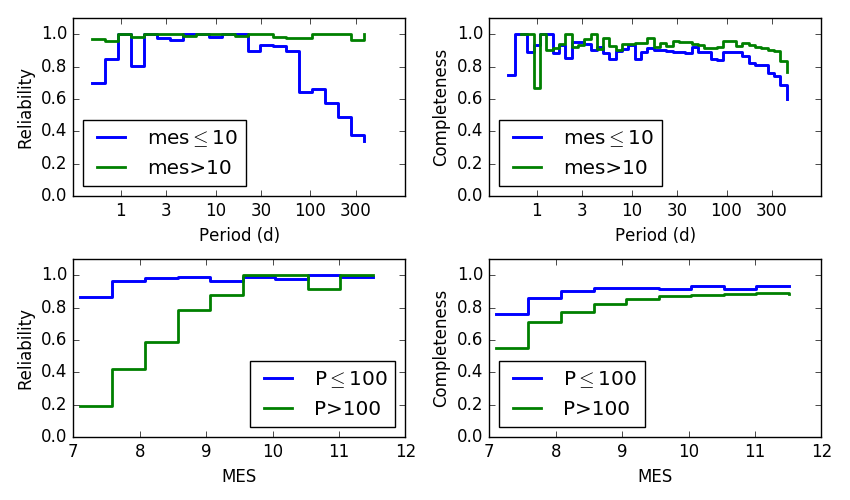
\includegraphics[width=1.0\linewidth]{fig-compRel1D-PerMes.png}
  \caption{\label{f:1dcomparel} The completeness (right) and reliability (left) of the DR25 catalog plotted for various Period (top) and MES (bottom) bins.}
 \end{center}
 \end{figure*}


\begin{figure*}[h!]
\begin{center}
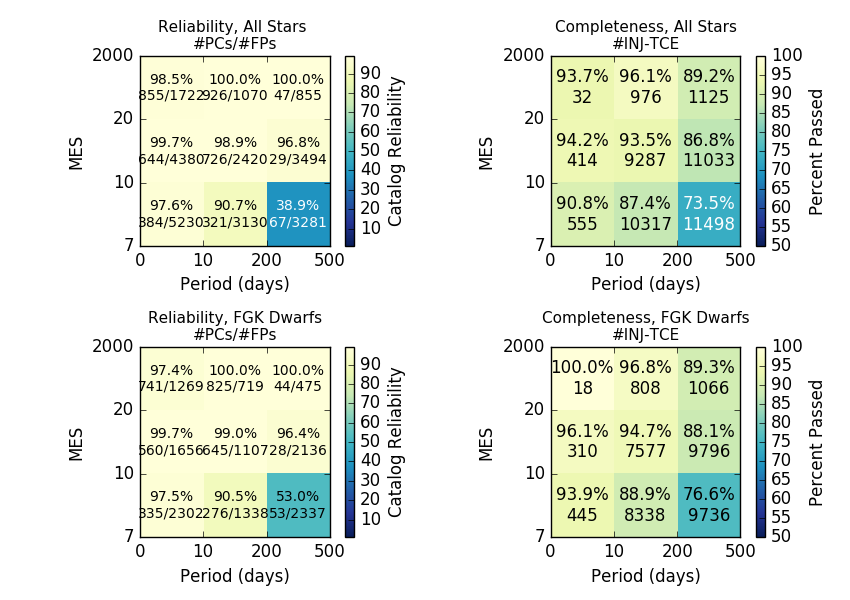
\includegraphics[width=0.9\linewidth]{fig-completeReliabilityCard.png}
\caption{\label{f:score} A coarse binning of the completeness and reliability across period and MES. On the left, the percentage for reliability is given in each box with the number of OPS-PCs and the number of OPS-FPs written below it.  On the right, the percentage for the completeness and the number of \injtce s for that box is given. The bottom two plots give the reliability and completeness just based on the FGK dwarf stars. }
\end{center}
\end{figure*}

\subsubsection{Use of the Scores}
We balanced the completeness and reliability
Include plot of changing score and how it changes C&R.

Plots we need to include here:
\begin{itemize}
\item[-] Completeness and reliability as a function of period, mes and number of transits. Bin the mes one by different period ranges. Bin the Period one by different MES (<15, 15-30, >30). Do number of transits by MES as well (<15, 15-30,>30.  

\item[-] Completeness and Reliability grids as MES and Period. very coarse. Might belong in the tuning section.

\item[-] Completeness and Reliabiltiy for the derived values.
Do 2d grids o Period vs radius, stellar temp vs radius and insolation flux vs radius.  The grids for completeness can be much finer than for reliability.  Either we show both as an interpolated contour, or we show completeness as just over resolved from the reliability. 

\item[-] Need to show how you can use the scores to adjust the completeness and reliability of the catalog. We have this plot.
\end{itemize}
